\section{Cryptographic hash algorithms}
\label{sec:hashalgs}
%
\index{Preimage resistance}
\index{Second-preimage resistance}
\index{Collision resistance}
A hash algorithm is a function assigning a given key to a value of fixed width $n$. Formally we define a hash function as $h: \{0, 1\}^* \rightarrow \{0, 1\}^n$. Hash functions in cryptography have to fulfill three requirements%
~\cite[2]{Cry02}:
%
\begin{description}
  \item[Preimage resistance] It is computationally infeasible to find a preimage
    $x$ for any given $y$ such that $h(x) = y$.
  \item[Second-preimage resistance] It is computationally infeasible to find a
    second preimage $x'$ for any given $x$ such that $h(x) = h(x')$ with $x \neq x'$.
  \item[Collision resistance] It is computationally infeasible to find two preimages
    $x$ and $x'$ such that $h(x) = h(x')$ with $x \neq x'$.
\end{description}

\section{SAT-based attacks}
\label{sec:sat_attacks}
%
% REMARK: https://github.com/vegard/sat2013-cryptocompo
Every year, new \gls{sat} solvers in the \gls{sat} competition~\cite{Sat21} emerge and use new techniques to improve upon solving problems in real-world applications, combinatorial hard and random problems.

SAT-based attacks on cryptographic hash functions describe the approach to represent a hash function in \gls{cnf} and solve the equation system with a \gls{sat} solver to look for preimages and collisions. Prior work in this field was done including:

\index{XOR clauses}
\begin{itemize}
  \item
Ekawat Homsirikamol, Paweł Morawiecki, Marcin Rogawski and Marian Srebrny~\cite{Cry04} evaluated the security margin of SHA-3 candidates. On the one hand they applied brute-force attacks to perform preimage attacks\footnote{The authors point out that an easy modification leads to a second preimage or collision attack.} and on the other hand they compare the number of broken rounds to the total number of rounds in the given cryptographic system. The first task can be subdivided into 3 parts: Generation of the CNF formula, fixing the hash and its padding bits in the formula and running a \gls{sat} solver on the generated CNF. They conclude that all five SHA-3 contest finalists have substantially bigger security margins than the SHA-256 and SHA-1 standards in regards of SAT-based attacks.
  \item
A paper ``Extending SAT Solvers to Cryptographic Problems'' by Mate Soos, Karsten Nohl and Claude Castelluccia~\cite{Cry06} builds the foundation of \cmsat{}; the \gls{sat} solver used in this bachelor's thesis. It describes a possible extension of the input algebra for XOR operations. Cryptographic primitives often use XOR operations and the authors expect performance improvements for SAT-based attacks using Gaussian elimination. \cmsat{}~2.9.10 was used in our implementation which natively uses \emph{XOR clauses}. Release \cmsat{} 3.0 discarded XOR clauses, but they returned in release 4.0.
  \item
Dejan Jovanović and Predrag Janičić~\cite{Sat03} described a framework to transform a hash algorithm implementation into a SAT problem instance. They use C++'s operator overloading to replace the semantics of the operators with the corresponding boolean ones. When transforming the problem into a CNF, they used Tseitin's Definitional Normal Form with linear growth of size rather than an exponential approach which is taken in this thesis. They concluded that a whole MD4 or MD5 instance cannot be evaluated with their implementation, but the problem can be scaled down by reducing the size of the input message or reducing the number of rounds. The paper has a very similar motivation, but this thesis targets differential cryptanalysis.
  \item
Gaëtan Leurent, Nicky Mouha and Bart Preneel~\cite{Sat10}\cite{Sat11} use the same differential characteristics theory used throughout this document. Gaëtan Leurent describes his design for a similar automated search; this document uses the one described in~\cite{Cry07}. Nicky Mouha and Bart Preneel also explain their own search strategies. In their usecase they try to increase the ``weight'' of differential characteristics. A SAT solver is used to determine whether a particular differential characteristic of a given weight exists. The encoding was not discussed explicitly and a Simple Theorem Prover solved their problem to create a CNF for a given equation. These papers are especially interesting to discuss search strategies and encoding approaches for hash algorithms.
\end{itemize}

\section{Differential cryptanalysis}
\label{sec:differential}
\index{Differential cryptanalysis}
%
\begin{figure}[t]
  \begin{center}
    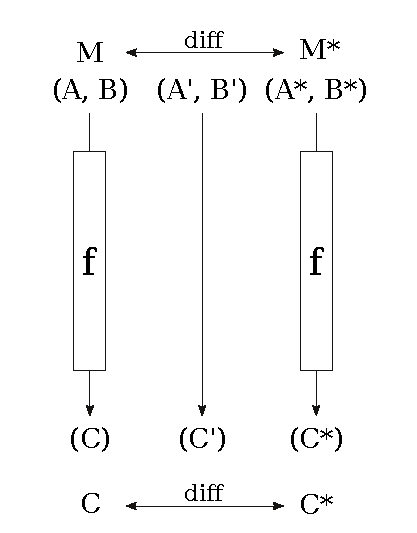
\includegraphics{img/diff_cryptanalysis.pdf}
    \caption{Two evaluation instances in differential cryptanalysis and their difference.}
    \label{fig:diff_cryptanalysis}
  \end{center}
\end{figure}

\index{Evaluation instances}
In \emph{differential cryptanalysis} we consider the difference between \emph{evaluation instances}. Assuming a hash function $f$ maps some input $M$ (derived from two parameters $A$ and $B$) to some output $C$, the difference between those instances in every step of the evaluation of the function $f$ is of interest for us. In Figure~\ref{fig:diff_cryptanalysis} an example with two instances $M$ and $M^*$ is illustrated.

Xiaoyun Wang successfully reduced the complexity of MD4, the original RIPEMD design and MD5 in 2005~\cite{Cry10} which made differential cryptanalysis popular in the research community.

In our thesis we want to discuss how differential characteristics can be encoded in boolean algebra. Fabio Massacci was the first to apply SAT research to cryptographic problems and coined the name \emph{logical cryptanalysis}. Our implementation specifically combines the fields of differential cryptanalysis and logical cryptanalysis.

In all following sections we always assume \emph{two} existing evaluation instances.

\subsection{Differential characteristics}
\label{sec:differential-characteristic}
%
In the following we want to describe a notation introduced by Christophe De Cannière and Christian Rechberger in their paper ``Finding SHA1-Characteristics: General Results and Applications''~\cite{Cry01}.

With our notation we want to represent the difference of single bits in those instances. In general 4 ($= 2^2$) cases must be distinguished, because of 2 values for 2 bits.

But in differentical cryptanalysis we often do not have enough information about the bits. We need to model insecurity. For example if the first bit is a zero, but the value of the second bit is unknown, 2 cases are possible ($0$ and $0$/$1$ for the first and second bit respectively). If we want to model ``the bits are different'' 2 cases are possible again. However if no knowledge about the bits' state is available, we have to consider all 4 cases.

\index{Bit condition}
\index{Free bit condition}
\index{Contradiction}
For the general notation we have to scale this picture. We have one bit in each evaluation instance and some of four different states are possible. This gives us 16 cases to distinguish: 1 case where no bit configuration is possible (the so-called \emph{contradiction}), 4 cases where only one configuration is possible, 6 cases with 2 configurations, 4 cases with 3 configurations and 1 configuration where every configuration is possible (the so-called \emph{free condition}). These cases are listed in Table~\ref{tab:bitconditions}. The most-left column specifies the so-called \emph{bit condition} representing a differential value. The superset relation between the bit conditions can be retrieved from the Galois lattice given in Figure~\ref{fig:bitconditions-lattice}.

% TODO: urgh, \yes and \no must not be bold. Or whatever to make the table beautiful
\begin{table}[p]
 \begin{center}
  \begin{tabular}{ccccc}
   \hline
    $(X_i, X_i^*)$ & (0, 0) & (1, 0) & (0, 1) & (1, 1) \\
   \hline \hline
         ?         & \yes   & \yes   & \yes   & \yes   \\
         -         & \yes   & \no    & \no    & \yes   \\
         x         & \no    & \yes   & \yes   & \no    \\
         0         & \yes   & \no    & \no    & \no    \\
         u         & \no    & \yes   & \no    & \no    \\
         n         & \no    & \no    & \yes   & \no    \\
         1         & \no    & \no    & \no    & \yes   \\
         \#        & \no    & \no    & \no    & \no    \\
         3         & \yes   & \yes   & \no    & \no    \\
         5         & \yes   & \no    & \yes   & \no    \\
         7         & \yes   & \yes   & \yes   & \no    \\
         A         & \no    & \yes   & \no    & \yes   \\
         B         & \yes   & \yes   & \no    & \yes   \\
         C         & \no    & \no    & \yes   & \yes   \\
         D         & \yes   & \no    & \yes   & \yes   \\
         E         & \no    & \yes   & \yes   & \yes   \\
   \hline
  \end{tabular}
  \caption[Bit conditions table]{Bit conditions table (most-left column specifies symbol).}
  \label{tab:bitconditions}
 \end{center}
\end{table}
\begin{figure}[p]
 \begin{center}
  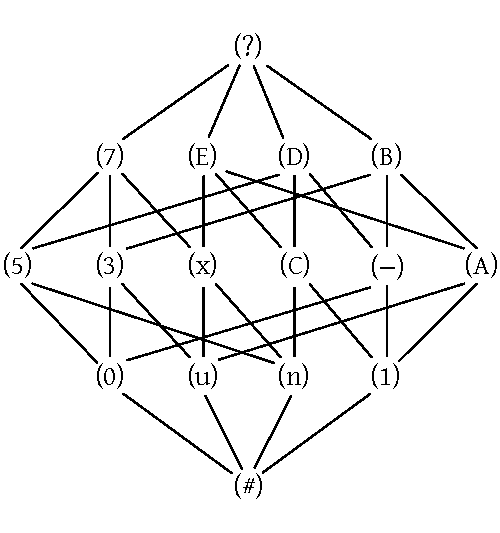
\includegraphics{img/bit_condition_lattice.pdf}
  \caption{Galois lattice of bit conditions.}
  \label{fig:bitconditions-lattice}
 \end{center}
\end{figure}

\index{Differential characteristic}
\index{Bitslice}
\index{Differential word}
In conclusion we introduced a notation to describe which bit configurations for two bits are possible in a certain state. A \emph{differential characteristic} represents a certain state of a hash algorithm in differential cryptanalysis. It is a list of bit conditions often represented as a matrix for better readability. A \emph{bitslice} is a column in a given differential characteristic. Analogously a \emph{differential word} is a row in a given differential characteristic.

\section{Evaluating differential characteristics}
\label{sec:diffchar-examples}
%
Several popular hash algorithms are built using the ARX architecture\footnote{The MD5, SHA-1 and SHA-2 hash algorithms follow the ARX design principle.}. One of the letters in the name refers to the XOR operation taking two or more arguments. The XOR operator returns true iff the number of arguments with value true is odd.

Let's consider a single bitslice with 2 input arguments and 1 output argument. The first input argument is \bc{1} and the second input argument is \bc{0}. It's important that \bc{1} and \bc{0} are bit conditions and therefore describe the state of 2 instances. For these particular bit conditions the values of both instances are the same: 1 and 0 respectively.
%
\begin{figure}[t]
  \begin{center}
    \begin{subfigure}[b]{0.23\textwidth}
      \begin{diffchar}
        A: 1 \\
        A: 0 \\
        S: 1
      \end{diffchar}
      \caption{SAT}
      \label{dc:xor1}
    \end{subfigure}%
    \begin{subfigure}[b]{0.23\textwidth}
      \begin{diffchar}
        A: 1 \\
        A: 0 \\
        S: ?
      \end{diffchar}
      \caption{SAT}
      \label{dc:xor2}
    \end{subfigure}%
    \begin{subfigure}[b]{0.23\textwidth}
      \begin{diffchar}
        A: 0001 \\
        A: 1010 \\
        S: 1011
      \end{diffchar}
      \caption{SAT}
      \label{dc:xor3}
    \end{subfigure}%
    \begin{subfigure}[b]{0.23\textwidth}
      \begin{diffchar}
        A: C\textendash{}\textendash{}? \\
        A: 3xx0 \\
        S: x?x?
      \end{diffchar}
      \caption{SAT}
      \label{dc:xor4}
    \end{subfigure}
    \caption{Examples for satisfiable differential characteristics (XOR operation).}
    \label{dc:xor-examples}
  \end{center}
\end{figure}
\begin{figure}[t]
  \begin{center}
    \begin{diffchar}
      A: BC0 \\
      A: 501 \\
      S: \textendash{}10
    \end{diffchar}
    \caption{An unsatisfiable differential characteristic (XOR operation).}
    \label{dc:xor-faulty}
  \end{center}
\end{figure}
%
Figure~\ref{dc:xor-examples} shows examples for satisfiable differential characteristics. If we apply the XOR operation on each bitslice, the output value does correspond to the given bit condition. Correspondence here means that any possible outcome of the function is part of the specified output argument. It is the hash algorithm's responsibility to define which arguments an operation is applied to. Here we assume a simple algorithm which applies XOR bitslice-by-bitslice.

In Figure~\ref{dc:xor1} a one as result in both instance is satisfiable for the XOR operation. In Figure~\ref{dc:xor2} we also have a satisfiable result, because \bc{?} is a superset of \bc{1}. Figure~\ref{dc:xor3} just illustrates the simultaneous application of the XOR operation to each bitslice of the differential characteristic. Figure~\ref{dc:xor4} provides more complex examples. For the second bitslice (from the right) the XOR operation applied to an input argument of equal values in both instances and an input argument with different values, the result will always be a difference between both instances. The third bitslice shows again a superset relation between \bc{?} and \bc{x}. In the fourth bitslice we also have to distinguish 4 cases (\bc{C} and \bc{3} can be 2 cases each) and if we evaluate the result, the bits in both instances will always be different.

A bit condition taken twice as input arguments to XOR is always \bc{0}. If a contradiction occurs in an input argument, the result is a contradiction. In Figure~\ref{dc:xor-faulty} an unsatisfiable differential characteristic is given. It is unsatisfiable, because some application of the XOR operation does not result in the specified bit condition; actually all applications will fail. The second bitslice is unsatisfiable, because if \bc{C} represents a 0 in the first instance and a 1 in the second instance, the application of XOR will return a 0 and 1 in each instance respectively which is not covered by the bit condition \bc{1}. The third bitslice has two input arguments which actually allows any possible result and relation between the values in each instance. Thus the bit condition \bc{-} is too strict.

Evaluating the satisfiability of a differential characteristic is the main requirement to enable our automated search.

\section{\nltool}
\label{sec:nltool}
%
\nltool{} is a framework for differential cryptanalysis. It provides various hash algorithm implementations and also allows to run partial subsets (like steps or rounds as defined by the particular hash algorithm). It implements a search algorithm trying to derive knowledge about some differential state of the hash algorithm evaluation. This propagation is a crucial task of the tool and this implementation improves upon existing ones. The tool and the details of the search got introduced in the paper~\cite[293]{Cry07}. For our implementation it is important to distinguish between two states within the search:

\begin{description}
  \item[Initialization]
    At initialization the hash algorithm (to be used) is known and the structure of the differential characteristic can be retrieved. The value of any bit condition is not yet available.
  \item[Update BitCondition]
    In the update step the values of the differential characteristic are provided and the final decision about satisfiability of the characteristic can be made.
\end{description}

Finding the best paths to derive new knowledge about the state is an open research topic. Differential paths are described in the master thesis ``Cryptanalysis of MD4'' by Martin Schläffer~\cite{Cry15} and an application of the tool for an attack is given by the paper ``Collision Attacks on the Reduced Dual-Stream Hash Function RIPEMD-128''~\cite{Cry08}.

\section{Automated search}
\label{sec:automated-search}
%
The search strategy applied to SHA-256 is a more sophisticated version than the one proposed by~\cite[10]{Cry01} and was proposed in the paper ``Finding SHA-2 Characteristics: Searching Through a Minefield of Contradictions''~\cite[298]{Cry07}:
\begin{quote}
Let \emph U be the set of all \texttt{`?'} and \texttt{`x'}, then repeat the following until U is empty.
\begin{enumerate}
  \item Pick randomly a bit in in \emph U.
  \item Impose a \texttt{`-'} for a \texttt{`?'} or randomly a sign (\texttt{`u'} or \texttt{`n'}) for \texttt{`x'}.
  \item Compute the propagation.
  \item If a contradiction is detected start backtracking, else apply additional checks.
  \item Continue with step 1 if all checks passed, if not start backtracking.
  \item If the decision bit is \texttt{`x'} try the second choice of the sign or if the decision bit \texttt{`?'} impose a \texttt{`x'}
  \item If still a contradiction occurs mark bit as critical.
  \item Jump back until the critical bit ca will be resolved.
  \item Continue with step 1.
\end{enumerate}
\end{quote}

\index{Overlapping bits}
The interesting point here is that the SAT solver implementation provides better propagation results. In the initialization step the reused values are known and the SAT solver implementation only creates boolean variables for values whenever they occur the first time. \emph{Overlapping bit} detection for two-bit conditions (as mentioned in \cite[296]{Cry07}) is an improvement of \nltool{} provided in this implementation. Overlapping bits are bit conditions which are used twice in a differential characteristic (and thus within the hash algorithm). So they always have the same value.

\section{Testcases for the Addition and Sigma function}
\label{sec:add-sigma-testcases}
%
Tables~\ref{dc:tcs-addition} and \ref{dc:tcs-sha2} list various testcases for the Addition and Sigma function and their satisfiability state. The Addition function uses carry bits\footnote{Denoted by a differential word C.} whose values are used in the next bitslice and is defined by

\index{Addition function}
\begin{minipage}{0.48\textwidth}
  \begin{align*}
    s_0 &= a_0 \oplus b_0 \\
    c_1 &= a_0 \land b_0 \\
    s_1 &= a_1 \oplus b_1 \oplus c_1 \\
    c_2 &= (a_1 \land b_1) \lor (b_1 \land c_1) \lor (c_1 \land a_1)
  \end{align*}
\end{minipage}
\begin{minipage}{0.48\textwidth}
  \begin{align*}
    s_2 &= a_2 \oplus b_2 \oplus c_2 \\
    c_3 &= (a_2 \land b_2) \lor (b_2 \land c_2) \lor (c_2 \land a_2) \\
    s_3 &= a_3 \oplus b_3 \oplus c_3
  \end{align*}
\end{minipage}

The Sigma function is defined by
\index{Sigma function (SHA-2)}
\begin{align*}
    b_0 &= a_1 \oplus a_2 \oplus a_3 \\
    b_1 &= a_2 \oplus a_3 \oplus a_0 \\
    b_2 &= a_3 \oplus a_0 \oplus a_1 \\
    b_3 &= a_0 \oplus a_1 \oplus a_2
\end{align*}

$a_0$ refers to the most-right value of the differential word A using zero-based indexing. $a_1$, $b_0$ and others are defined respectively.

So in conclusion both functions reuse bits of the previous bitslice. Previous implementations could not detect such \emph{overlapping bits} and this detection provides a better propagation result in the automated search, because cases where the overlapping bit condition differs must not be tested.

%Figure~\ref{fig:sigma-vis} tries to visualize the reuse of the values in the function with colors.
%
%\begin{figure}[t]
%  \begin{center}
%    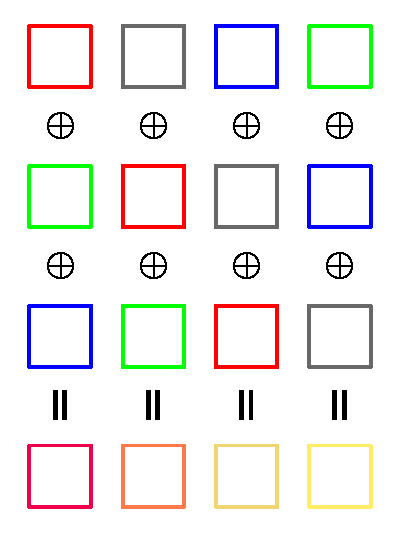
\includegraphics{img/sigma.pdf}
%    \caption{Values of the Sigma function visualized.}
%    \label{fig:sigma-vis}
%  \end{center}
%\end{figure}

\begin{figure}[p]
  \begin{center}
    \begin{subfigure}[b]{0.23\textwidth}
      \begin{diffchar}
        A: 0011 \\
        B: 0101 \\
        S: 1000
      \end{diffchar}
      \caption{SAT}
      \label{dc:tcs-addition-1}
    \end{subfigure}
    \begin{subfigure}[b]{0.23\textwidth}
      \begin{diffchar}
        A: 0011 \\
        B: 0101 \\
        S: 0000
      \end{diffchar}
      \caption{UNSAT}
      \label{dc:tcs-addition-2}
    \end{subfigure}
    \begin{subfigure}[b]{0.23\textwidth}
      \begin{diffchar}
       A: \textendash{}\textendash{}\textendash{}x \\
       B: \textendash{}\textendash{}\textendash{}x \\
       S: ???x
      \end{diffchar}
      \caption{UNSAT}
      \label{dc:tcs-addition-3}
    \end{subfigure}
    \begin{subfigure}[b]{0.23\textwidth}
      \begin{diffchar}
        A: \textendash{}\textendash{}\textendash{}x \\
        B: \textendash{}\textendash{}\textendash{}x \\
        S: ???\textendash{}
      \end{diffchar}
      \caption{SAT}
      \label{dc:tcs-addition-4}
    \end{subfigure}
  \end{center}%

  \begin{center}
    \begin{subfigure}[b]{0.23\textwidth}
      \begin{diffchar}
        A: \textendash{}\textendash{}\textendash{}x \\
        B: \textendash{}\textendash{}\textendash{}x \\
        S: ????
      \end{diffchar}
      \caption{SAT}
      \label{dc:tcs-addition-5}
    \end{subfigure}
    \begin{subfigure}[b]{0.23\textwidth}
      \begin{diffchar}
        A: \textendash{}\textendash{}\textendash{}\textendash{} \\
        B: \textendash{}\textendash{}\textendash{}x \\
        S: x\textendash{}??
      \end{diffchar}
      \caption{UNSAT}
      \label{dc:tcs-addition-6}
    \end{subfigure}
    \begin{subfigure}[b]{0.23\textwidth}
      \begin{diffchar}
        A: \textendash{}\textendash{}\textendash{}x \\
        B: \textendash{}\textendash{}\textendash{}x \\
        S: x???
      \end{diffchar}
      \caption{SAT}
      \label{dc:tcs-addition-7}
    \end{subfigure}
  \end{center}
  \caption{Testcases for the ADD2 function (addition with 2 input arguments).}
  \label{dc:tcs-addition}
\end{figure}

\begin{figure}[p]
  \begin{center}
    \begin{subfigure}[b]{0.23\textwidth}
      \begin{diffchar}
        A: \textendash{}\textendash{}\textendash{}\textendash{} \\
        S: 0000
      \end{diffchar}
      \caption{SAT}
      \label{dc:tcs-sigma-1}
    \end{subfigure}
    \begin{subfigure}[b]{0.23\textwidth}
      \begin{diffchar}
        A: 7C\textendash{}3 \\
        S: \textendash{}3u?
      \end{diffchar}
      \caption{SAT}
      \label{dc:tcs-sigma-2}
    \end{subfigure}
  \end{center}

  \begin{center}
    \begin{subfigure}[b]{0.23\textwidth}
      \begin{diffchar}
        A: \textendash{}\textendash{}\textendash{}x \\
        S: 0000
      \end{diffchar}
      \caption{UNSAT}
      \label{dc:tcs-sigma-3}
    \end{subfigure}
    \begin{subfigure}[b]{0.23\textwidth}
      \begin{diffchar}
        A: xxxx \\
        S: 0000 \\
      \end{diffchar}
      \caption{UNSAT}
      \label{dc:tcs-sigma-4}
    \end{subfigure}
    \begin{subfigure}[b]{0.23\textwidth}
      \begin{diffchar}
        A: 0uCD \\
        S: ADC7 \\
      \end{diffchar}
      \caption{SAT}
      \label{dc:tcs-sigma-5}
    \end{subfigure}
  \end{center}
  \caption{Testcases for the SHA-2 Sigma function.}
  \label{dc:tcs-sha2}
\end{figure}

We will discuss the differential characteristic~\ref{dc:tcs-addition-4} in more detail as an example. We have two evaluation instances and the first bitslice claims that the two input arguments for the Addition function are different between the instances. In this case the output arguments are equal. Table~\ref{tab:tcs-addition-4-first-bitslice} lists all possible cases. In any case the column $s_0$ indicates that the values in both instances are equal. Thus the bit condition \bc{-} is a valid assumption. At the same time we observe that we cannot derive much information about the state of $c_1$, which has three possible cases $(0, 0)$, $(0, 1)$ and $(1, 0)$. The case $(1, 1)$ is excluded. If we continue deducing the bit conditions for the Addition operation we observe that the carry bit makes it impossible to draw a conclusion for any $s$-value like for $s_0$. As a result this differential characteristic is valid.

\begin{table}[t]
  \begin{center}
    \begin{tabular}{l|cccc}
     \hline \hline
                 & $a_0$ & $b_0$ & $s_0$ & $c_1$ \\
     \hline
      instance 1 &   0   &   0   &   0   &   0  \\
      instance 2 &   1   &   1   &   0   &   1  \\
     \hline
      instance 1 &   0   &   1   &   1   &   0  \\
      instance 2 &   1   &   0   &   1   &   0  \\
     \hline
      instance 1 &   1   &   0   &   1   &   0  \\
      instance 2 &   0   &   1   &   1   &   0  \\
     \hline
      instance 1 &   1   &   1   &   0   &   1  \\
      instance 2 &   0   &   0   &   0   &   0  \\
     \hline \hline
    \end{tabular}
    \caption{List of possibilities for the bits of the first bitslice in Figure~\ref{dc:tcs-addition-4}.}
    \label{tab:tcs-addition-4-first-bitslice}
  \end{center}
\end{table}

